%%%%%% Compile using latex, then dvips, then ps2pdf %%%%%%%%%%%%%

\documentclass{beamer}

%\documentclass[handout]{beamer}

%\includeonlyframes{current}

\mode<presentation>
{
%  \usetheme{Warsaw}
%  \usetheme{Frankfurt}
%  \usetheme{Singapore}
\usetheme{Boadilla}
}

\usepackage{times}
\usepackage[T1]{fontenc}
\usepackage[english]{babel}
\usepackage[latin1]{inputenc}

\usepackage{tikz}
\usepackage{pgflibraryshapes}
\usetikzlibrary{shapes}

\usepackage{graphics}
%\usepackage[draft]{graphics}

\usepackage{xspace}
\usepackage{amsmath}
\usepackage{bm}
\usepackage{pgfpages}
\usepackage{fancybox}
\usepackage{threeparttable}
\usepackage{bbding}
\usepackage{booktabs}

\setbeamersize{text margin left=0.5cm,text margin right=0.5cm}

\setbeamercolor{equation.box}{fg=blue,bg=yellow!50!white}
\setbeamercolor{postit}{fg=black,bg=yellow!75!white}


%\graphicspath{{D:/teaching/figs/}}

%Additional commands



% Abbreviations for equations and lists

\newenvironment{shitemize}{
\begin{itemize}
\setlength{\parskip}{0pt} \setlength{\itemsep}{10pt}
\setlength{\parsep}{0pt}
%\setlength{\baselineskip}{7mm}
\setlength{\baselineskip}{8mm} }{\end{itemize}}

\newcommand{\bi}{\begin{itemize}}
\newcommand{\ei}{\end{itemize}}
\newcommand{\I}{\item}

% for a bulleted list nested within another bulleted list
\newcommand{\nestedbi}{\begin{itemize}}
\newcommand{\nestedei}{\end{itemize}}

% for a bulleted list with larger spacing between lines
\newcommand{\bibig}{\begin{itemize}}
\newcommand{\eibig}{\end{itemize}}

\newenvironment{senumerate}{\begin{enumerate}
\setlength{\parskip}{0pt} \setlength{\itemsep}{3pt}
\setlength{\parsep}{0pt} \setlength{\baselineskip}{10mm}
}{\end{enumerate}}


\newenvironment{shenumerate}{\begin{enumerate}
\setlength{\parskip}{0pt}
\setlength{\itemsep}{2pt}
\setlength{\parsep}{0pt}
}{\end{enumerate}}

\newcommand{\beq}{\begin{equation}}
\newcommand{\eeq}{\end{equation}}

\newcommand{\bea}{\begin{eqnarray}}
\newcommand{\eea}{\end{eqnarray}}

\newcommand{\beas}{\begin{eqnarray*}}
\newcommand{\eeas}{\end{eqnarray*}}

\newcommand{\ben}{\begin{enumerate}}
\newcommand{\een}{\end{enumerate}}

\newcommand{\beqs}{\begin{eqnarray*}}
\newcommand{\eeqs}{\end{eqnarray*}}



% for a section heading
\newcommand{\sect}[1]{
     {\large{\bf #1}}\vspace{0.05in}}

% for a subsection heading
\newcommand{\subsect}[1]{{\bf #1}\vspace{0.05in}}

% for a subsubsection heading
\newcommand{\subsubsect}[1]{{\it{#1}}\vspace{0.05in}}

% Misc.
\newcommand{\etal}{{\it et al.}}
\newcommand{\winbugs}{{\sc WinBUGS }}

% spaces
\newcommand{\negsp}{\vspace{-0.5cm}}
\newcommand{\possp}{\vspace{0.5cm}}

% Maths
%\usepackage{D:/teaching/maths}     % my maths style file

\newcommand{\EE}{\mathrm{I\!E}}  %% Expectation
\newcommand{\VV}{\mathrm{Var}} %% Variance

\newcommand{\bbeta}{\boldsymbol{\beta}}
\newcommand{\btheta}{\boldsymbol{\theta}}
\newcommand{\bnu}{\boldsymbol{\nu}}
\newcommand{\pmat}{\boldsymbol{p}}
\newcommand{\bx}{\boldsymbol{x}}

\newcommand{\pr}{\ensuremath{\mathbb{P}}}

\newcommand{\sis}{{\sigma^2}}

\newcommand{\E}{\mathbb{E}}

\newcommand{\No}{\text{Normal}}
\newcommand{\Ga}{\text{Gamma}}
\newcommand{\Uni}{\text{Uniform}}
\newcommand{\Bin}{\text{Binomial}}

\newcommand{\pari}{\hspace{\parindent}}

\title[Bayesian Statistics (AIMS)]
{\Huge{Lecture \vspace{5mm}\\Introduction to Markov Chain Monte Carlo methods}}

\author[Nathan Green]
{}
\date[]
{}


\begin{document}

\begin{frame}[t]
  \titlepage

\end{frame}

\frame{
\frametitle{Learning Objectives}
After this session students should be able to:\vspace{2mm}
\begin{itemize}
  \item Describe MCMC simulation methods\vspace{2mm}
  \item Compare and contrast MCMC and MC methods learnt in the previous lectures\vspace{2mm}
  \item Describe the main methods available to check for convergence of MCMC simulations\vspace{2mm}
  \item Explain the role of MC error in determining the effective sample size of an MCMC simulation\vspace{2mm}
\end{itemize}
}
%%%%%%%%%%%%%%%%%%%%%%%%%%%%%%%%%%%%%%%%%%%%%%%%%%%%%%%%%%%%%%%%%%%%%%%%


\frame{
\frametitle{Outline}
\begin{itemize}
  \item \alert{Why Bayesian methods?}\vspace{2mm}
  \item \alert{ Likelihood, prior and posterior: how are they connected?}\vspace{2mm}
  \item \alert{Bayes's theorem and example in diagnostic setting}\vspace{2mm}
  \item \alert{Inference on proportions: Binomial-Beta models}\vspace{2mm}
   \item Inference on continuous data: Normal-Normal models\vspace{2mm}
  \item Inference on count data: Poisson-Gamma models

\end{itemize}
}

%%%%%%%%%%%%%%%%%%%%%%%%%%%%%%%%%%%%%%%%%%%%%%%%%%%%%%%%%%%%%%%%%%%%%%%%

\begin{frame}[t]
\frametitle{Why Bayesian methods?}

\bibig
\I Bayesian methods have been widely applied in many areas:\vspace{1mm}
   \nestedbi
   \I medicine / epidemiology\vspace{1mm}
   \I genetics\vspace{1mm}
   \I ecology\vspace{1mm}
   \I environmental sciences\vspace{1mm}
   \I social and political sciences\vspace{1mm}
   \I finance\vspace{1mm}
   \I archaeology\vspace{1mm}
   \I .....\vspace{2mm}
   \nestedei
\I Motivations for adopting Bayesian approach vary:\vspace{1mm}
   \nestedbi
   \I natural and coherent way of thinking about science and learning\vspace{1mm}
   \I pragmatic choice that is suitable for the problem in hand\vspace{1mm}
   \nestedei
\eibig
\end{frame}

%%%%%%%%%%%%%%%%%%%%%%%%%%%%%%%%%%%%%%%%%%%%%%%%%%%%%%%%%%%%%%%%%%%%%%%%

\begin{frame}[t]

\frametitle{Example}

A clinical trial is carried out to collect evidence about an
unknown \lq treatment effect'

\vspace{5mm}

\alert{Conventional analysis}\vspace{1mm}
\bi
\I p-value for $H_0$: treatment effect is zero\vspace{1mm}
\I Point estimate and CI as summaries of  size of treatment effect\vspace{1mm}
\ei
Aim is to learn what this trial tells us about the treatment effect

\vspace{5mm}

\alert{Bayesian analysis}\vspace{1mm}
\bi
\I Inference is based on probability statements summarising the posterior
   distribution of the treatment effect\vspace{1mm}
\ei
Asks: \lq how should this trial change our opinion about
   the treatment effect?'
\end{frame}

%%%%%%%%%%%%%%%%%%%%%%%%%%%%%%%%%%%%%%%%%%%%%%%%%%%%%%%%%%%%%%%%%%%%%%%%

\begin{frame}[t]

\frametitle{Components of a Bayesian analysis}

The Bayesian analyst needs to explicitly state\vspace{1mm}
\bi
\I a reasonable opinion concerning the plausibility
   of different values of the treatment effect
  {\it excluding} the evidence from the trial
  (the \alert{prior distribution})\vspace{1mm}
\I the support for different values of the treatment
   effect based {\it solely} on data from the
   trial (the \alert{likelihood}),\vspace{1mm}
\ei
and to combine these two sources to produce\vspace{1mm}
\bi
\I a final opinion about the treatment effect
   (the \alert{posterior distribution})
\ei

\vspace{2mm}
The final combination is done using Bayes theorem (and only simple rules of probability), which essentially weights the likelihood from the trial with the relative plausibilities defined by the prior distribution

\vspace{2mm}
One can view the Bayesian approach as a formalisation of the process
of learning from experience
\end{frame}

%%%%%%%%%%%%%%%%%%%%%%%%%%%%%%%%%%%%%%%%%%%%%%%%%%%%%%%%%%%%%%%%%%%%%%%%

\begin{frame}[t]

\frametitle{Bayesian inference: the posterior distribution}

Posterior distribution forms basis for all inference --- can
be summarised to provide\vspace{2mm}
\bibig
\I point and interval estimates of Quantities of Interest (QOI), e.g. treatment effect, small area estimates, $\hdots$\vspace{2mm}
\I point and interval estimates of any function of the parameters\vspace{2mm}
\I probability that QOI (e.g. treatment effect) exceeds a critical threshold\vspace{2mm}
\I prediction of QOI in a new unit\vspace{2mm}
\I prior information for future experiments, trials, surveys, $\hdots$\vspace{2mm}
\I inputs for decision making\vspace{2mm}
\I $\hdots$
\eibig
\end{frame}

%%%%%%%%%%%%%%%%%%%%%%%%%%%%%%%%%%%%%%%%%%%%%%%%%%%%%%%%%%%%%%%%%%%%%%%%

\begin{frame}[t]

\frametitle{Bayes theorem and its link with Bayesian inference}

\subsect{Bayes' theorem}

\bi
\I Provable from probability axioms\vspace{2mm}
\I Let $A$ and $B$ be events, then

$$ p(A|B) = \frac{ p(B|A) p(A) } {p(B)}$$\vspace{1mm}

\I Similarly 
$$ p(B|A) = \frac{ p(A| B) p(B)}{p(A)}$$ \vspace{1mm}

\I If $A_i$ is a set of mutually exclusive and exhaustive events
({\it i.e.} $ p( \bigcup\limits_i A_i ) = \sum\limits_i p(A_i) = 1 $), then

$$ p(A_i|B) = \frac{ p(B|A_i) p(A_i) } {\sum\limits_j p(B|A_j) p(A_j) }$$
\ei
\end{frame}

%%%%%%%%%%%%%%%%%%%%%%%%%%%%%%%%%%%%%%%%%%%%%%%%%%%%%%%%%%%%%%%%%%%%%%%%


 \begin{frame}[t]

\frametitle{Example: use of Bayes theorem in diagnostic testing}

A new HIV test is claimed to have \lq\lq 95\% sensitivity and 98\% specificity''

In a population with an HIV prevalence of 1/1000, what
is the chance that a patient testing positive actually has HIV?

\bi
\I Let $A$ be the event that patient is truly HIV positive,
$\overline{A}$ be the event that they are truly HIV negative
\I Let $B$ be the event that they test positive
\I We want $p(A|B)$
\I \lq\lq95\% sensitivity'' means that $p(B|A) = .95$
\I \lq\lq98\% specificity'' means that $p(B|\overline{A}) = .02$
\I Now Bayes theorem says $$ p(A|B) = \frac{ p(B|A) p(A) } {p(B|A) p(A) + p(B|\overline{A}) p(\overline{A}) }$$
\I Hence  $ p(A|B) = \frac{ .95 \times .001 } {.95 \times  .001 + .02 \times.999 } = .045 $
\I Thus over 95\% of those testing positive will, in fact, not have HIV
\ei
\end{frame}


%%%%%%%%%%%%%%%%%%%%%%%%%%%%%%%%%%%%%%%%%%%%%%%%%%%%%%%%%%%%%%%%%%%%%%%%

\begin{frame}[t]

\frametitle{Comments}

\bibig
\I Our intuition is poor when processing probabilistic evidence\vspace{1mm}
\I The vital issue is {\it how should this test result change our belief
   that patient is HIV positive?}\vspace{1mm}
\I The disease prevalence can be thought of as a {\it \lq prior'} probability ($p$ = 0.001)\vspace{1mm}
\I Observing a positive result causes us to modify this probability to $p$ = 0.045.
   This is our {\it \lq posterior'} probability that patient is HIV positive.\vspace{1mm}
\I Bayes theorem applied to {\it observables} (as in diagnostic testing)
   is uncontroversial and established\vspace{1mm}
\I More controversial is the use of Bayes theorem in general statistical analyses,
   where {\it parameters} are the unknown quantities, and their prior distribution
   needs to be specified --- this is \alert{Bayesian inference}
\eibig
\end{frame}

%%%%%%%%%%%%%%%%%%%%%%%%%%%%%%%%%%%%%%%%%%%%%%%%%%%%%%%%%%%%%%%%%%%%%%%%

\begin{frame}[t]

\frametitle{Bayesian inference}

Makes fundamental distinction between
\begin{itemize}
\item Observable quantities $y$, i.e.~the data\vspace{2mm}
\item Unknown quantities $\theta$\vspace{1mm}
\begin{itemize}
\item $\theta$ can be statistical parameters, missing data, mismeasured data $\hdots$\vspace{1mm}
\item[$\rightarrow$] parameters are treated as random variables\vspace{1mm}
\item[$\rightarrow$] in the Bayesian framework, we make probability statements about model parameters\vspace{2mm}
\end{itemize}
\item[!] in the Frequentist framework, parameters are fixed non-random quantities and the probability statements concern the data\vspace{2mm}
\end{itemize}
As with any statistical analysis, we start building a model which specifies $p(y \mid \theta)$\\ \vspace{2mm}

This is the \alert{likelihood}, which relates all variables into a \alert{\lq full probability model'}
\end{frame}

%%%%%%%%%%%%%%%%%%%%%%%%%%%%%%%%%%%%%%%%%%%%%%%%%%%%%%%%%%%%%%%%%%%%%%%%





\frame{
\frametitle{Bayesian inference [continued]}
From a Bayesian point of view\vspace{1mm}
\begin{itemize}
\item  $\theta$ is unknown so should have a \alert{probability distribution} reflecting
     our uncertainty about it before seeing the data\vspace{1mm}
     \begin{itemize}
     \item[$\rightarrow$] need to specify a \alert{prior distribution} $p(\theta)$\vspace{2mm}
     \end{itemize}
\item $y$ is known so we should condition on it\vspace{1mm}
     \begin{itemize}
     \item[$\rightarrow$] use Bayes theorem to obtain conditional probability distribution
      for unobserved quantities of interest given the data:
      \alert{$$p(\theta \mid y)= \frac{ p(\theta)\, p(y \mid \theta)}
                         {\int  p(\theta)\,p(y \mid \theta)\,d\theta}
	\propto p(\theta)\,p(y \mid \theta)$$}
        \item[] This is the \alert{posterior distribution}\vspace{2mm}
     \end{itemize}
\end{itemize}
The prior distribution $p(\theta)$, expresses our uncertainty about $\theta$ \alert{before} seeing the data\vspace{2mm}

The posterior distribution $p(\theta \mid y)$, expresses our uncertainty about $\theta$ \alert{after} seeing the data
}

%%%%%%%%%%%%%%%%%%%%%%%%%%%%%%%%%%%%%%%%%%%%%%%%%%%%%%%%%%%%%%%%%%%%%%%%
\section{Inference on proportion}
\frame{

\frametitle{Example: Inference on proportions}

\begin{itemize}
\item Recall example from Lecture 2 where we consider early investigation of a new drug\vspace{2mm}
\item Experience with similar compounds has suggested that
      response rates between 0.2 and 0.6 could be feasible\vspace{2mm}
\item We interpreted this as a distribution with mean = 0.4, standard deviation
      0.1 and showed that a Beta(9.2,13.8) distribution has these
      properties\vspace{2mm}
\item Suppose we now treat $n=20$ volunteers with the compound and
      observe $y=15$ positive responses\vspace{2mm}
\end{itemize}
}
%%%%%%%%%%%%%%%%%%%%%%%%%%%%%%%%%%%%%%%%%%%%%%%%%%%%%%%%%%%%%%%%%%%%%%%%
\frame{
\frametitle{Identifying the different model components}

\textbf{Likelihood (distribution of the data):}\\ \vspace{1mm}
\begin{itemize}
\item Assuming patients are independent, with common unknown response rate $\theta$,
leads to a binomial likelihood
\begin{eqnarray*}
p(y \mid  n, \theta) &=&
 \left( \begin{array}{c} n \\ y \end{array} \right) \theta^y (1-\theta)^{n-y}
 \; \propto \; \theta^y (1-\theta)^{n-y}
\end{eqnarray*}
\end{itemize}

\vspace{5pt}

\textbf{$\theta$  needs to be given a continuous prior distribution:}\\ \vspace{1mm}
\begin{itemize}
\item Recall from Lecture 2 that the Beta distribution is used in these cases
\begin{eqnarray*}
\theta & \sim & \hbox{Beta}(a, b)\\[5pt]
p(\theta) &=& \frac{\Gamma (a+b)}{\Gamma (a) \Gamma(b)} \; \theta^{a-1} (1-\theta)^{b-1}
\end{eqnarray*}
\end{itemize}
}
%%%%%%%%%%%%%%%%%%%%%%%%%%%%%%%%%%%%%%%%%%%%%%%%%%%%%%%%%%%%%%%%%%%%%%%%
\frame{
\frametitle{Combining prior and likelihood}

Combining the Binomial likelihood and the Beta prior gives the following posterior distribution
\alert{\begin{eqnarray*}
 p(\theta \mid y, n)  & \propto & p(y \mid \theta, n) p(\theta)\\ [8pt]
& \propto & \theta^y (1-\theta)^{n-y} \theta^{a-1} (1-\theta)^{b-1}\\[8pt]
& = & \theta^{y+a-1} (1-\theta)^{n-y+b-1}
\end{eqnarray*}
}

The posterior is still a Beta distribution (with different parameters):

\begin{center}
$p(\theta \mid y, n)  \propto  \hbox{Beta}(y+a, \; n-y+b)$\end{center}

\begin{center}\framebox{\pr{\textcolor{red}{\large When the prior and posterior come from the same family of distributions
the prior is said to be {\bf conjugate} to the likelihood}}}\end{center}
}
%%%%%%%%%%%%%%%%%%%%%%%%%%%%%%%%%%%%%%%%%%%%%%%%%%%%%%%%%%%%%%%%%%%%%%%%
\frame{
\frametitle{Prior, likelihood and posterior for Drug example}

\begin{center}
%\rotatebox{-90}{\scalebox{0.5}{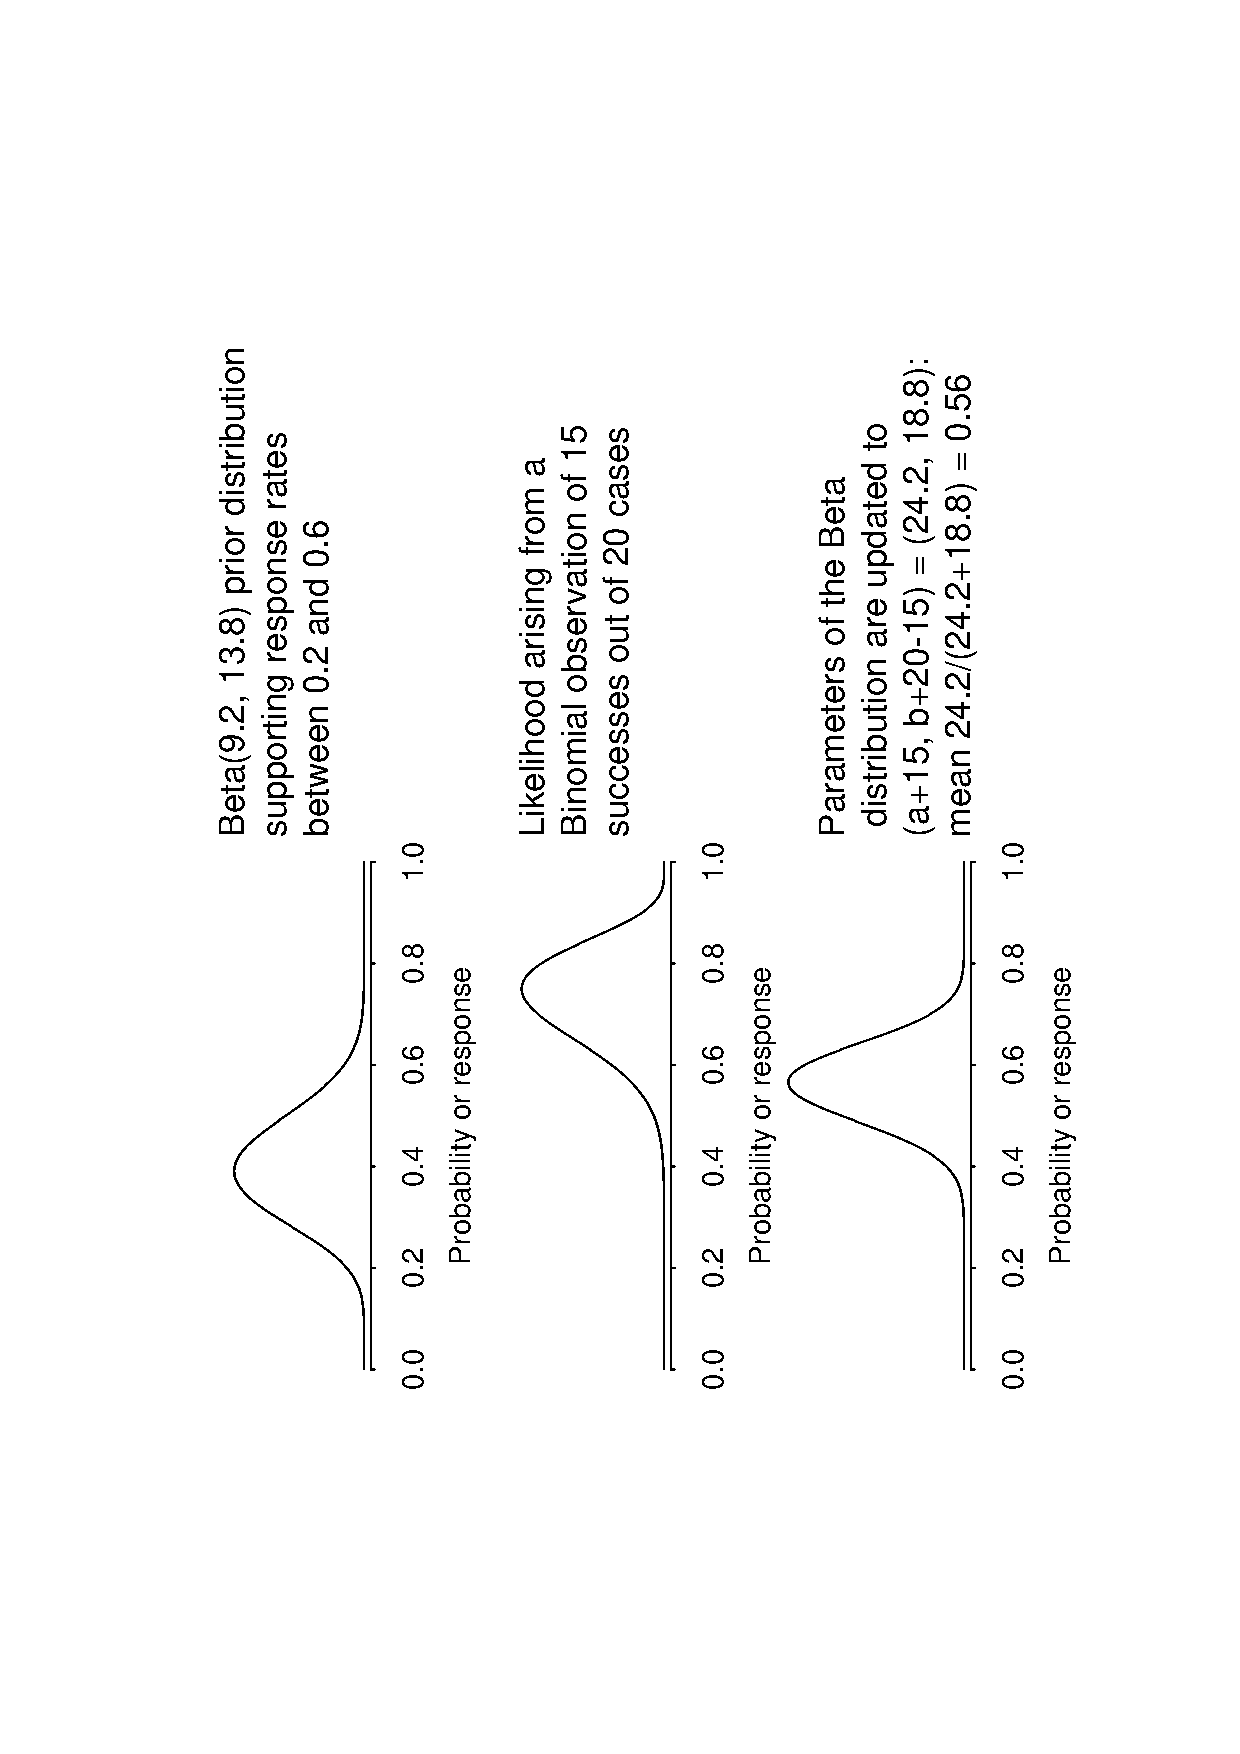
\includegraphics{beta-binomial}}}
\end{center}
\vspace{-20mm}
\centerline{\scalebox{0.5}{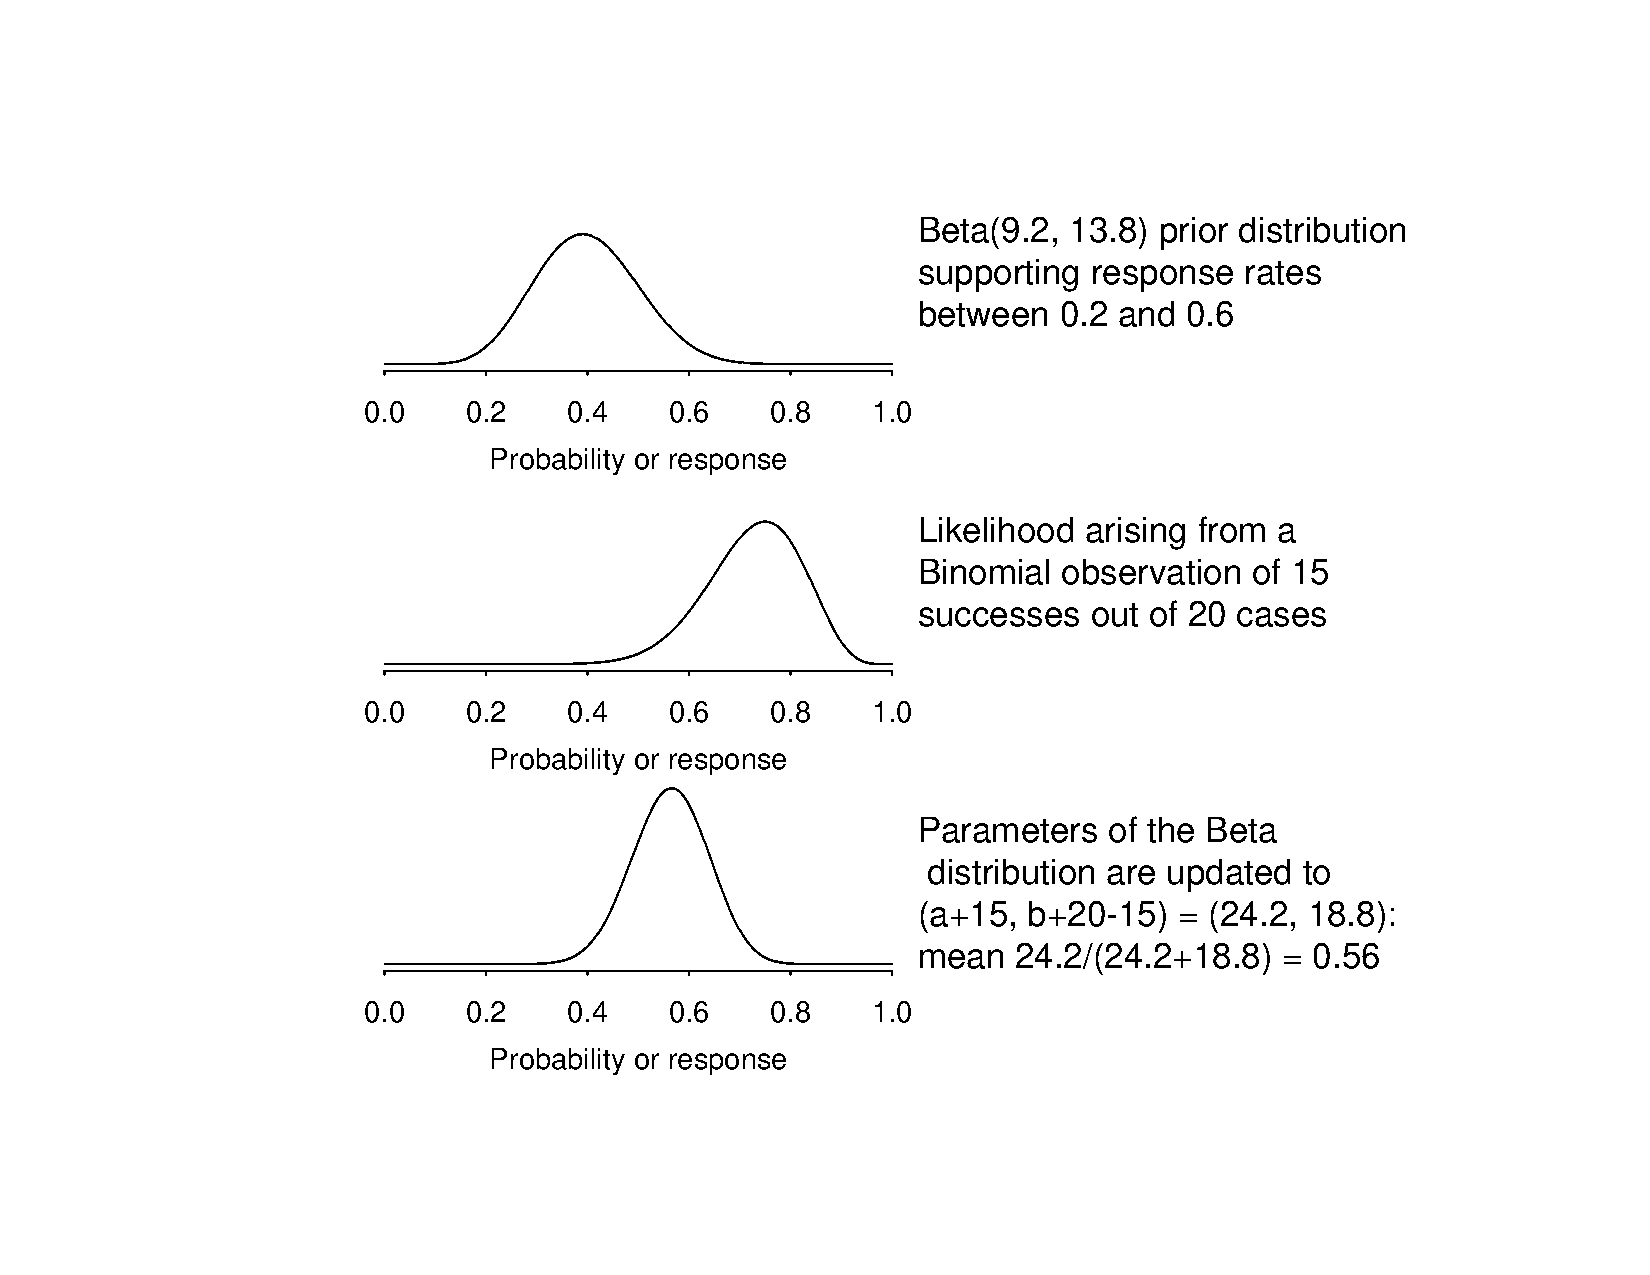
\includegraphics{Figures/beta-binomial.pdf}}}
}
%%%%%%%%%%%%%%%%%%%%%%%%%%%%%%%%%%%%%%%%%%%%%%%%%%%%%%%%%%%%%%%%%%%%%%%%

\begin{frame}[containsverbatim]

\frametitle{Posterior inference using simulation methods}

\bibig
\I In the Drug example, we have calculated the posterior
   distribution in closed form\vspace{1mm}
   \bi
   \I this is possible because we are using conjugate priors\vspace{2mm}
   \ei
\item No need to explicitly calculate posterior if using simulation methods\vspace{2mm}
\item In OpenBUGS just specify prior and likelihood separately\vspace{2mm}
\item OpenBUGS contains algorithms to evaluate the posterior given
(almost) arbitrary specification of prior and likelihood\vspace{1mm}
  \begin{itemize}
  \item posterior doesn't need to be closed form\vspace{1mm}
  \item but can recognise conjugacy when it exists, in which case OpenBUGS will sample
        directly from the closed form posterior
  \end{itemize}
\end{itemize}

\end{frame}
%%%%%%%%%%%%%%%%%%%%%%%%%%%%%%%%%%%%%%%%%%%%%%%%%%%%%%%%%%%%%%%%%%%%%%%%
\begin{frame}[containsverbatim]

\frametitle{\winbugs code for drug model}

\bibig
\item Drug model in OpenBUGS syntax:
\small
\begin{verbatim}
model {
 theta ~ dbeta(9.2, 13.8) # prior distribution
 y     ~ dbin(theta, 20)  # sampling distribution
 y <- 15                  # data
}
\end{verbatim}\vspace{2mm}
\normalsize
\item Note that the only difference between this code and the code for implementing the drug model for predicting $y$ seen in Lecture 2 is that we now specify the observed value of $y$ from our study \vspace{2mm}
\item \winbugs automatically knows that if any variables have observed values (i.e.~data) then these need to be conditioned on, and that posterior inference (rather than forward sampling) is required
\end{itemize}

\end{frame}
%%%%%%%%%%%%%%%%%%%%%%%%%%%%%%%%%%%%%%%%%%%%%%%%%%%%%%%%%%%%%%%%%%%%%%%%

\begin{frame}[containsverbatim]
\frametitle{Posterior Predictions for Drug example}

Now suppose we would consider continuing a development program if the drug
managed to achieve at least a further 25 successes out of $m$=40 future trials. How do we include this into the model?

\vspace{0.4cm}
\begin{tabular}{ccll}
$\theta$     &$\sim$ & ${\rm Beta}[a,b]$  &     prior distribution\\ [3pt]
$y$         &$\sim$ & ${\rm Binomial}[\theta,n] $       &  sampling distribution    \\ [3pt]
$y_{\rm pred}$    &$\sim$ & ${\rm Binomial}[\theta,m] $  &            predictive distribution \\ [3pt]
$P_{\rm crit}$    &$=$&  $P(y_{\rm pred}    \ge m_{\rm crit}    ) $
& Probability of exceeding critical threshold \\ [10pt]
\end{tabular}

In BUGS syntax:\vspace{-2mm}
{\fontsize{9}{9}\selectfont
\begin{verbatim}

# Model description
model {
  theta     ~ dbeta(a,b)              # prior distribution
  y         ~ dbin(theta,n)           # sampling distribution
  y.pred    ~ dbin(theta,m)           # predictive distribution
  P.crit   <- step(y.pred-mcrit+0.5)  # =1 if y.pred >= mcrit,
                                         0 otherwise
}
\end{verbatim}
}
\end{frame}

%%%%%%%%%%%%%%%%%%%%%%%%%%%%%%%%%%%%%%%%%%%%%%%%%%%%%%%%%%%%%%%%%%%%%%%%
\begin{frame}[containsverbatim]

\frametitle{Data files}

Data can be written after the model description, or held in a separate .txt or .odc file

{\fontsize{9}{9}\selectfont
\begin{verbatim}
 list( a = 9.2,    # parameters of prior distribution
  b = 13.8,
  y = 15,     # number of successes
  n = 20,     # number of trials
  m = 40,     # future number of trials
  mcrit = 25) # critical value of future successes
\end{verbatim}
}

Alternatively, in this simple example, we could have put all data and constants into model description:

{\fontsize{9}{9}\selectfont
\begin{verbatim}
model{
  theta     ~ dbeta(9.2,13.8)      # prior distribution
  y         ~ dbin(theta,20)       # sampling distribution
  y.pred    ~ dbin(theta,40)       # predictive distribution
  P.crit   <- step(y.pred-24.5)    # =1 if y.pred >= mcrit,
                                      0 otherwise
  y        <- 15
}
\end{verbatim}
}
\end{frame}
%%%%%%%%%%%%%%%%%%%%%%%%%%%%%%%%%%%%%%%%%%%%%%%%%%%%%%%%%%%%%%%%%%%%%%%

\frame{
\frametitle{Posterior and predictive distributions for Drug example}
\begin{center}
%\rotatebox{-90}{\scalebox{0.4}{\includegraphics{beta-binomial-pred.ps}}}
\end{center}
\vspace{-5mm}
\begin{small}
(a) Beta posterior distribution for $\theta$ after observing 15 successes in 20 trials\vspace{1mm}

(b) Predictive Beta-Binomial distribution of the number of successes
    $y_{pred}$ in the next 40 trials: mean 22.5 and standard deviation 4.3

%Suppose we would consider continuing a development program if the drug
%managed to achieve at least a further 25 successes out of these 40 future trials
%
%From Beta-binomial distribution, can calculate $P(\tilde{y}_{40} \ge 25) = 0.329$
\end{small}
\vspace{-20mm}
\centerline{\scalebox{0.5}{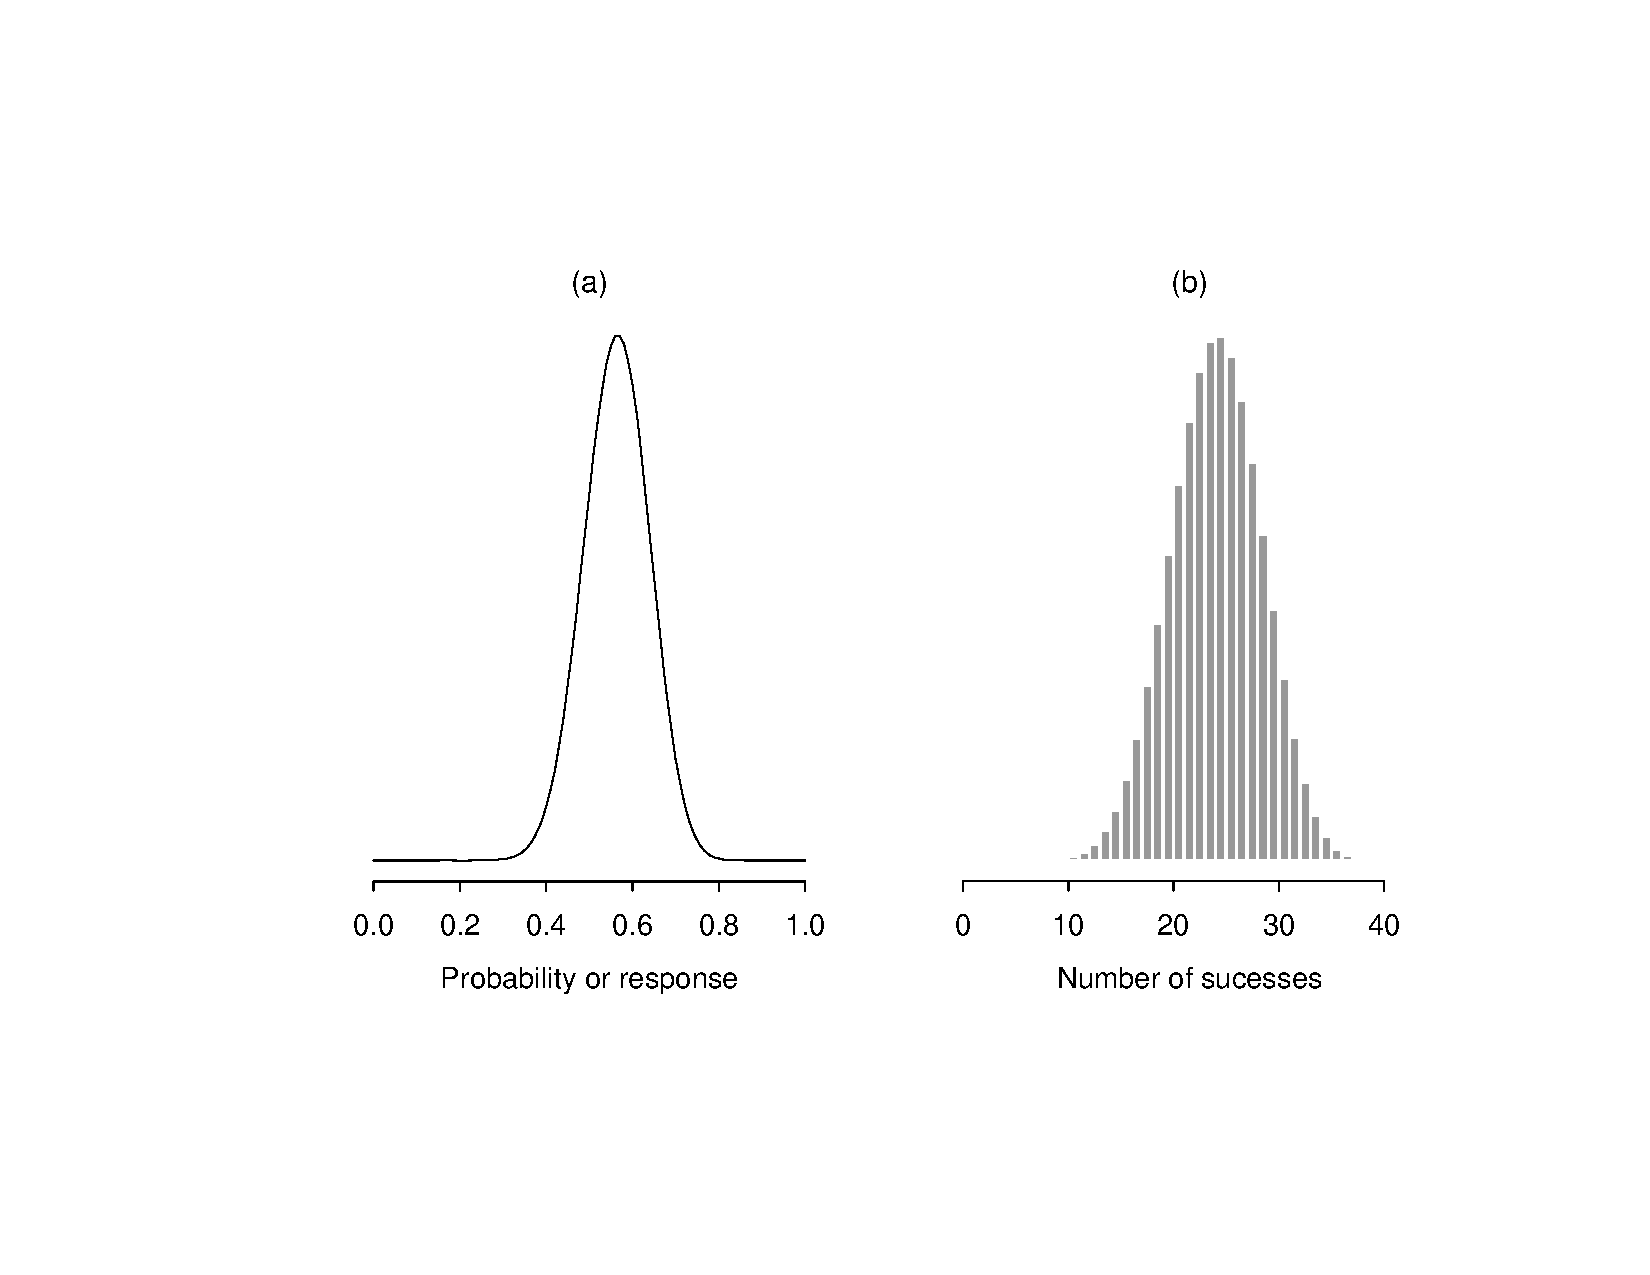
\includegraphics{Figures/beta-binomial-pred.pdf}}}
}
%%%%%%%%%%%%%%%%%%%%%%%%%%%%%%%%%%%%%%%%%%%%%%%%%%%%%%%%%%%%%%%%%%%%%%%%


\begin{frame}[containsverbatim]\frametitle{{\sc OpenBUGS} output and exact answers}
{\it{\sc OpenBUGS}}
{\fontsize{7}{7}\selectfont
\begin{verbatim}
node        mean     sd      MC error   2.5%    median   97.5%  start  sample
theta      0.5633   0.07458  4.292E-4   0.4139  0.5647  0.7051  1001   30000
y.pred     22.52    4.278    0.02356    14.0    23.0    31.0    1001   30000
P.crit     0.3273   0.4692   0.002631   0.0     0.0     1.0     1001   30000
\end{verbatim}
}

\centerline{\scalebox{0.45}{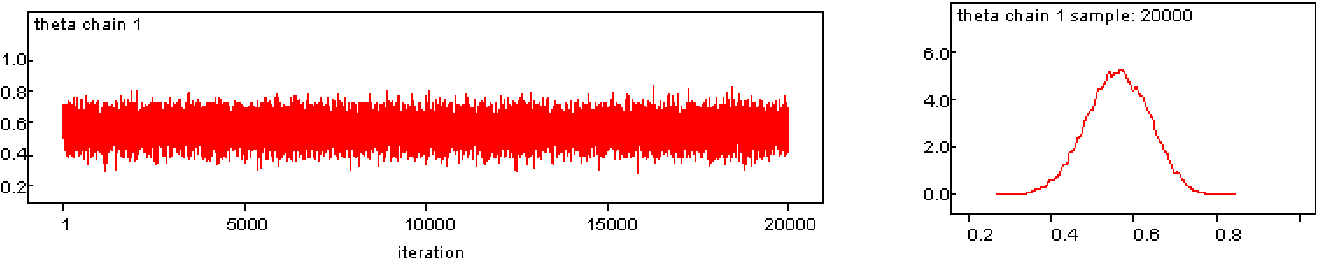
\includegraphics{Figures/drug-WB-plots.pdf}}}
%\begin{center}\rotatebox{-90}{\scalebox{0.4}{\vspace{-10pt}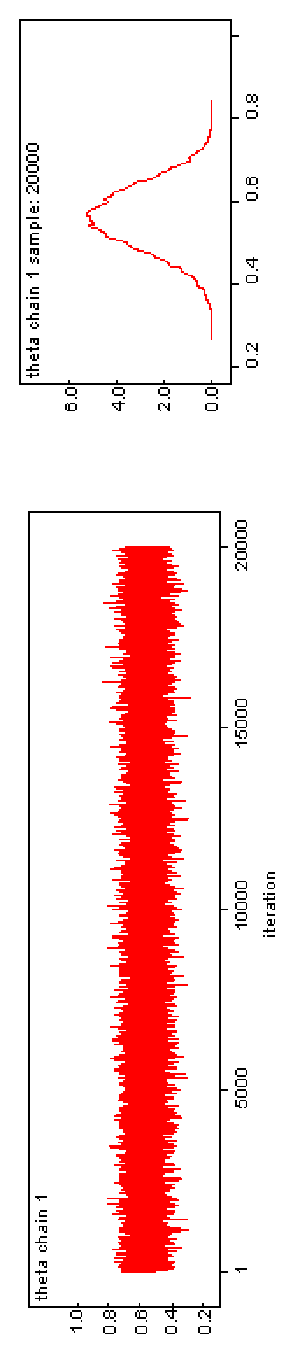
\includegraphics{drug-WB-plots.eps}}}\end{center}

{\it Exact answers from conjugate analysis}

\begin{itemize}
\item $\theta$:  mean 0.563 and standard deviation  0.075\vspace{1mm}
\item $y_{pred}$:  mean 22.51 and standard deviation  4.31\vspace{1mm}
\item Probability of at least 25:  0.329\vspace{2mm}
\end{itemize}

\end{frame}

%%%%%%%%%%%%%%%%%%%%%%%%%%%%%%%%%%%%%%%%%%%%%%%%%%%%%%%%%%%%%%%%%%%%%%%%
\frame{
\frametitle{Summary}
So far\vspace{2mm}
\begin{itemize}
  \item We have introduced the two components which play a key role in Bayesian analysis (prior and likelihood) and we have seen how to combine them to obtain the posterior distribution through Bayes' theorem\vspace{2mm}
  \item We have familiarised with conjugate models (when the prior and the posterior distribution come from the same family)\vspace{2mm}
  \item We have learnt about the Binomial-Beta model and seen how this can be applied in OpenBUGS
\end{itemize}
}



\end{document}




